\documentclass[hyperref=colorlinks]{beamer}
\mode<presentation>
\usetheme{iclpt}
\setbeamertemplate{navigation symbols}{}
\setbeamertemplate{headline}{
  \begin{beamercolorbox}[leftskip=.2cm,rightskip=.2cm,topskip=.2cm,ht=1.1cm,dp=0.1cm,wd=\textwidth]{institute in head/foot}
    
\includegraphics[height=1cm]{icl.pdf}
    \hfill
    \includegraphics[height=1cm]{../Pics/ATLAS-Logo-Square-Blue-RGB.png}
    
\includegraphics[height=1cm]{../Pics/CMS-Color.pdf}
  \end{beamercolorbox}
}
\setbeamertemplate{footline}{
  \begin{beamercolorbox}[ht=.35cm,dp=0.2cm,wd=\textwidth,leftskip=.3cm]{author in head/foot}%
    \begin{minipage}[c]{5cm}%
      \usebeamerfont{author in head/foot}
      \insertshortauthor 
      \insertshorttitle
    \end{minipage}\hfill%
    \hfill
    \insertframenumber{} / \ref{lastframe}
    %\hfill
    \begin{minipage}{6cm}
      \hfill
      %\insertshorttitle
    \end{minipage}
  \end{beamercolorbox}%
}

\definecolor{beamer@icdarkblue}{RGB}{0,51,102}
\definecolor{beamer@icmiddleblue}{RGB}{0,82,150} 
\definecolor{beamer@iclightblue}{RGB}{200,212,232}
\definecolor{beamer@icmiddlered}{RGB}{204,51,0}
\definecolor{beamer@iclightred}{RGB}{232,212,32}

\usepackage{tikz}
\usetikzlibrary{arrows,shapes,backgrounds}
\usepackage{color}
\usepackage{tabularx,colortbl}
\usepackage{graphicx}
\usepackage{pdfpages}
\usepackage{feynmp}
\usepackage{rotating}
\usepackage{moresize}
\usepackage{slashed}
\usepackage{xcolor,colortbl}
\DeclareGraphicsRule{*}{mps}{*}{}
\hypersetup{colorlinks=false}

\title[Latest results on invisibly decaying Higgs bosons]{\vspace{-0.2cm} Latest results on invisibly decaying Higgs bosons}
\author[P. Dunne]{Patrick Dunne - Imperial College London \\ on behalf of the ATLAS and CMS Collaborations \\ DM@LHC 2016 - 31/03/2016}
\titlegraphic{
  \vspace{-0.4cm}
  \begin{fmffile}{dmlhcfeyndiagstitle}
    \begin{fmfgraph*}(75,75)
      \fmfleft{i0,i2,ix,i3,i5}
      \fmfright{o0,o3,o1,o4,o6}
      \fmf{phantom,tension=4/3}{i2,v1,o3}
      \fmf{phantom,tension=4/3}{i3,v2,o4}
      \fmffreeze
      \fmf{gluon,tension=4/3}{i2,v1}
      \fmf{gluon,tension=4/3}{i3,v2}
      \fmf{fermion,tension=0}{v1,v2}
      \fmf{fermion,tension=2/3}{v2,v3,v1}
      \fmf{dashes}{v3,o1}
      \fmflabel{$g$}{i2}
      \fmflabel{$g$}{i3}
      \fmflabel{$H$}{o1}
    \end{fmfgraph*}    
    \hspace{.5cm}
    \begin{fmfgraph*}(75,75)
      \fmfleft{i1,i2}
      \fmfright{o1,o2,o3}
      \fmf{fermion}{i1,v1,o1}
      \fmf{fermion}{i2,v2,o3}
      \fmf{photon,label=$W,,Z$}{v1,v3}
      \fmf{photon,label=$W,,Z$}{v2,v3}
      \fmf{dashes}{v3,o2}
      \fmflabel{$q$}{i1}
      \fmflabel{$q$}{i2}
      \fmflabel{$q$}{o1}
      \fmflabel{$q$}{o3}
      \fmflabel{$H$}{o2}
    \end{fmfgraph*}
    \hspace{.5cm}
    \begin{fmfgraph*}(75,75)
      \fmfleft{i1,i2}
      \fmfright{o1,o2}
      \fmf{fermion}{i1,v1}
      \fmf{fermion}{v1,i2}
      \fmf{photon,label=$W,,Z$}{v1,v2}
      \fmf{photon}{v2,o1}
      \fmf{dashes}{v2,o2}
      \fmflabel{$q$}{i1}
      \fmflabel{$\bar{q}$}{i2}
      \fmflabel{$W,Z$}{o1}
      \fmflabel{$H$}{o2}
    \end{fmfgraph*}
  \end{fmffile}
  %% \begin{fmfgraph*}(100,70)
  %%         \fmfleft{i1,i2}
  %%         \fmfright{o1,o2,o3}
  %%         \fmf{fermion}{i1,v1,o1}
  %%         \fmf{fermion}{i2,v2,o3}
  %%         \fmf{phantom,tension=4/5}{v1,v2}
  %%         \fmffreeze
  %%         \fmf{photon,label=$W,,Z$}{v1,v3}
  %%         \fmf{photon,label=$W,,Z$}{v2,v3}
  %%         \fmf{dashes}{v3,o2}
  %%         \fmflabel{$q$}{i1}
  %%         \fmflabel{$q$}{i2}
  %%         \fmflabel{$q$}{o1}
  %%         \fmflabel{$q$}{o3}
  %%         \fmflabel{$H$}{o2}

  %%       \end{fmfgraph*}
}
\date{}
\begin{document}
\tikzstyle{every picture}+=[remember picture]
\tikzstyle{na} = [baseline=-.5ex]
\begin{fmffile}{dmlhcfeyndiags}


%??add ATLAS logo
  %TITLE PAGE
  %20 mins + 5 questions
  \section{Title}
  \begin{frame}
    \titlepage
  \end{frame}

  \begin{frame}
    \frametitle{Outline}
    \begin{block}{}
      \begin{itemize}
      \item How to search for invisibly decaying Higgs bosons:
      \item[-] direct and indirect searches
      \item Run 1 results from ATLAS and CMS
      \item Run 2 results from CMS
      \item Projections of future sensitivity
      \end{itemize}
    \end{block}
  \end{frame}

  \begin{frame}
    \frametitle{Why look for invisibly decaying Higgs bosons?}
    \vspace{-.3cm}
    \begin{columns}
      \column{1.06\textwidth}
    \begin{block}{Theoretical Motivations}
      \small
      \begin{itemize}
      \item All SM massive particles get their mass through Higgs boson couplings
      \item Why not dark matter?
      \end{itemize}
    \end{block}
    \end{columns}

    \vspace{-.2cm}    

    \begin{columns}
    \column{.55\textwidth}
    \begin{block}{Experimental motivation}
      \small
      \begin{itemize}
      \item Measurements of the Higgs boson made so far are impressive:
        \vspace{-.1cm}
      \item[-] Mass measured with 0.2\% error
      \item A lot of parameters are still relatively unconstrained:
        \vspace{-.1cm}
      \item[-] Limit on width is $\sim$4$\Gamma_{SM}$
      \item Plenty of room for Higgs boson couplings to dark matter
      \end{itemize}
    \end{block}
    \column{.45\textwidth}
    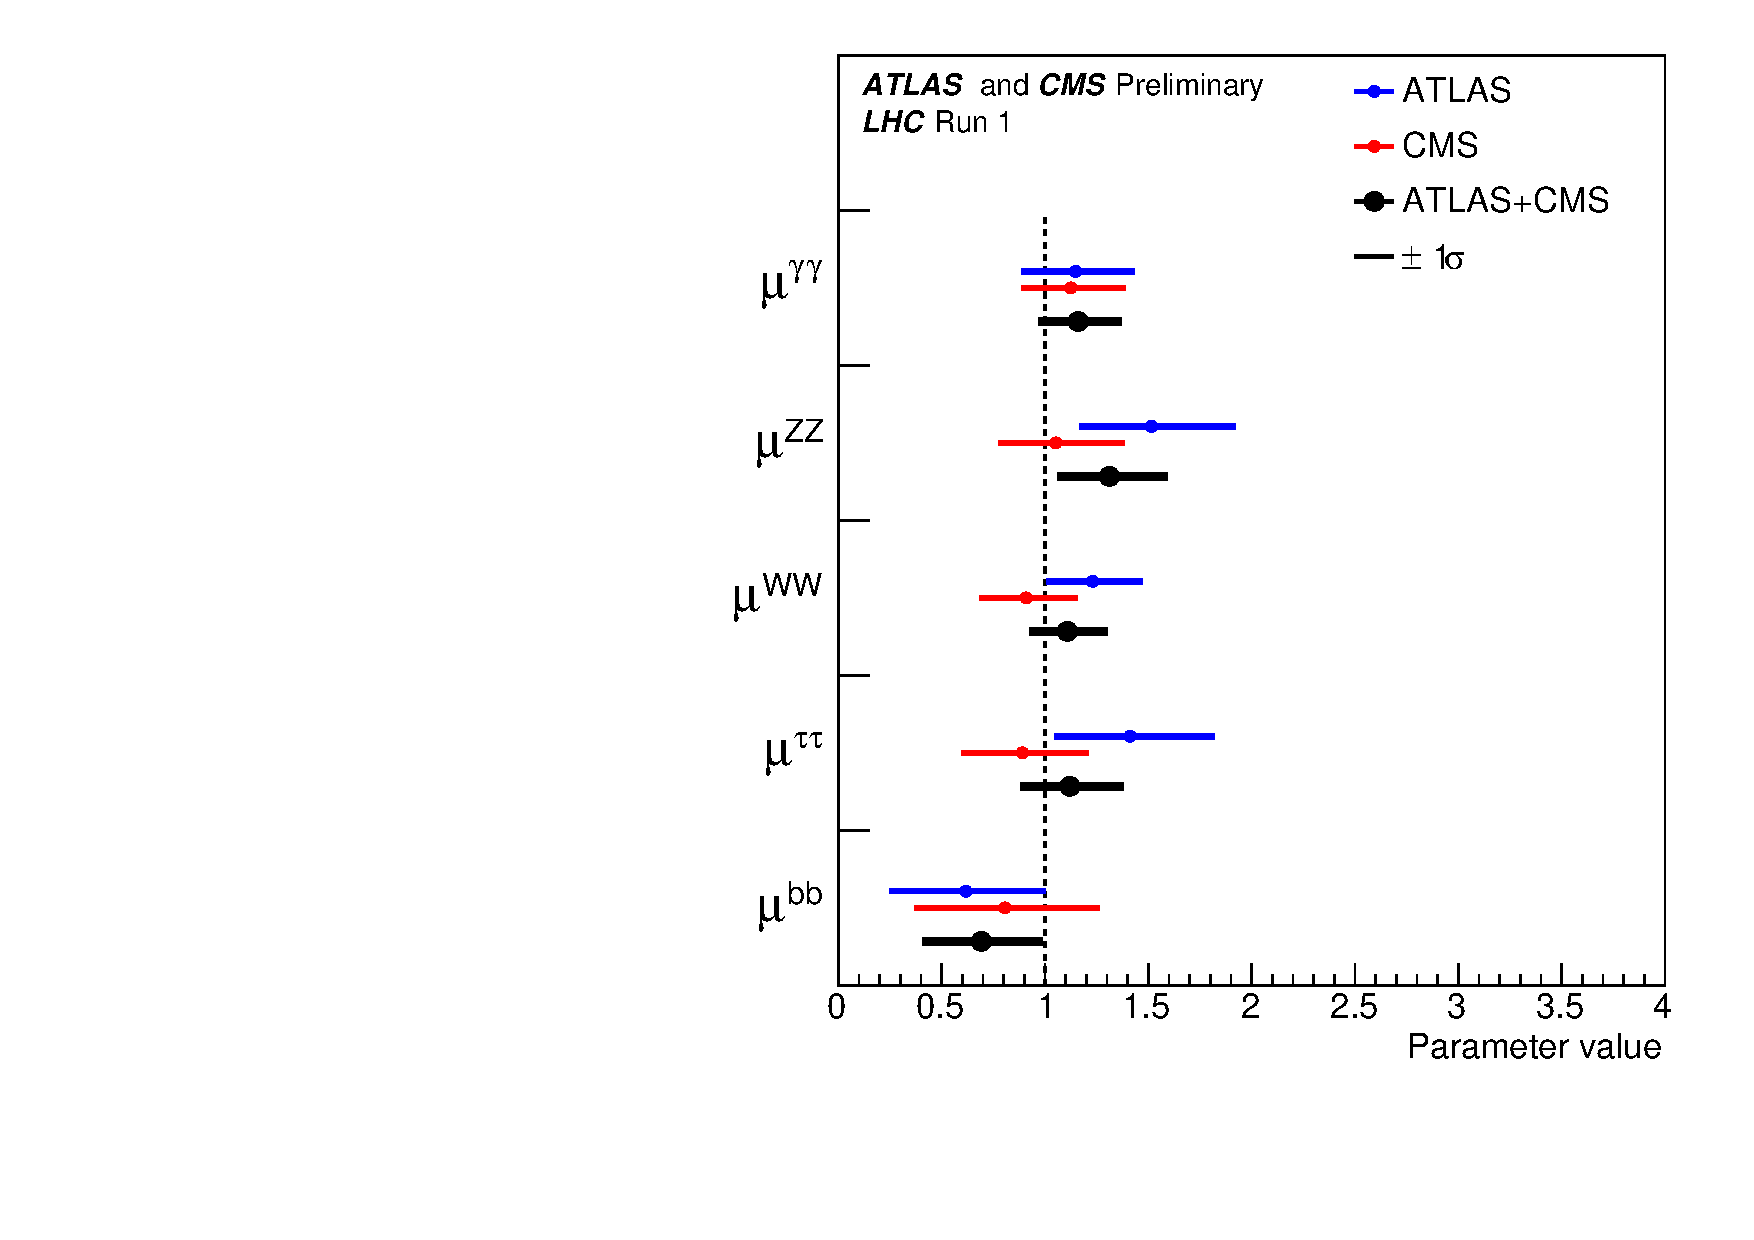
\includegraphics[width=\textwidth]{TalkPics/DM@LHC2016/CMS-PAS-HIG-15-002_Figure_012.pdf}
    \end{columns}
  \end{frame}

  \begin{frame}
    \frametitle{How to search for invisibly decaying Higgs bosons}
    \vspace{-.2cm}
    \begin{columns}
      \column{.5\textwidth}
      \begin{block}{Indirect searches}
        \begin{minipage}[t][.7\textheight][t]{\textwidth}
          \small
          \begin{itemize}
          \item Compare visible width to total width:
          \item[-] $\rm{BR}_{BSM}=\frac{\Gamma_{H}-\Gamma_{vis}}{\Gamma_{H}}$
          \item No measurement of $\Gamma_{H}$, need to make an assumption
          \item[-] Usually assume SM width
          \item ATLAS+CMS combination gives an observed (expected) limit on $\rm{BR}_{BSM}$ of 0.34 (0.35) at 95\% CL
          \end{itemize}
        \end{minipage}
      \end{block}
      \column{.5\textwidth}
      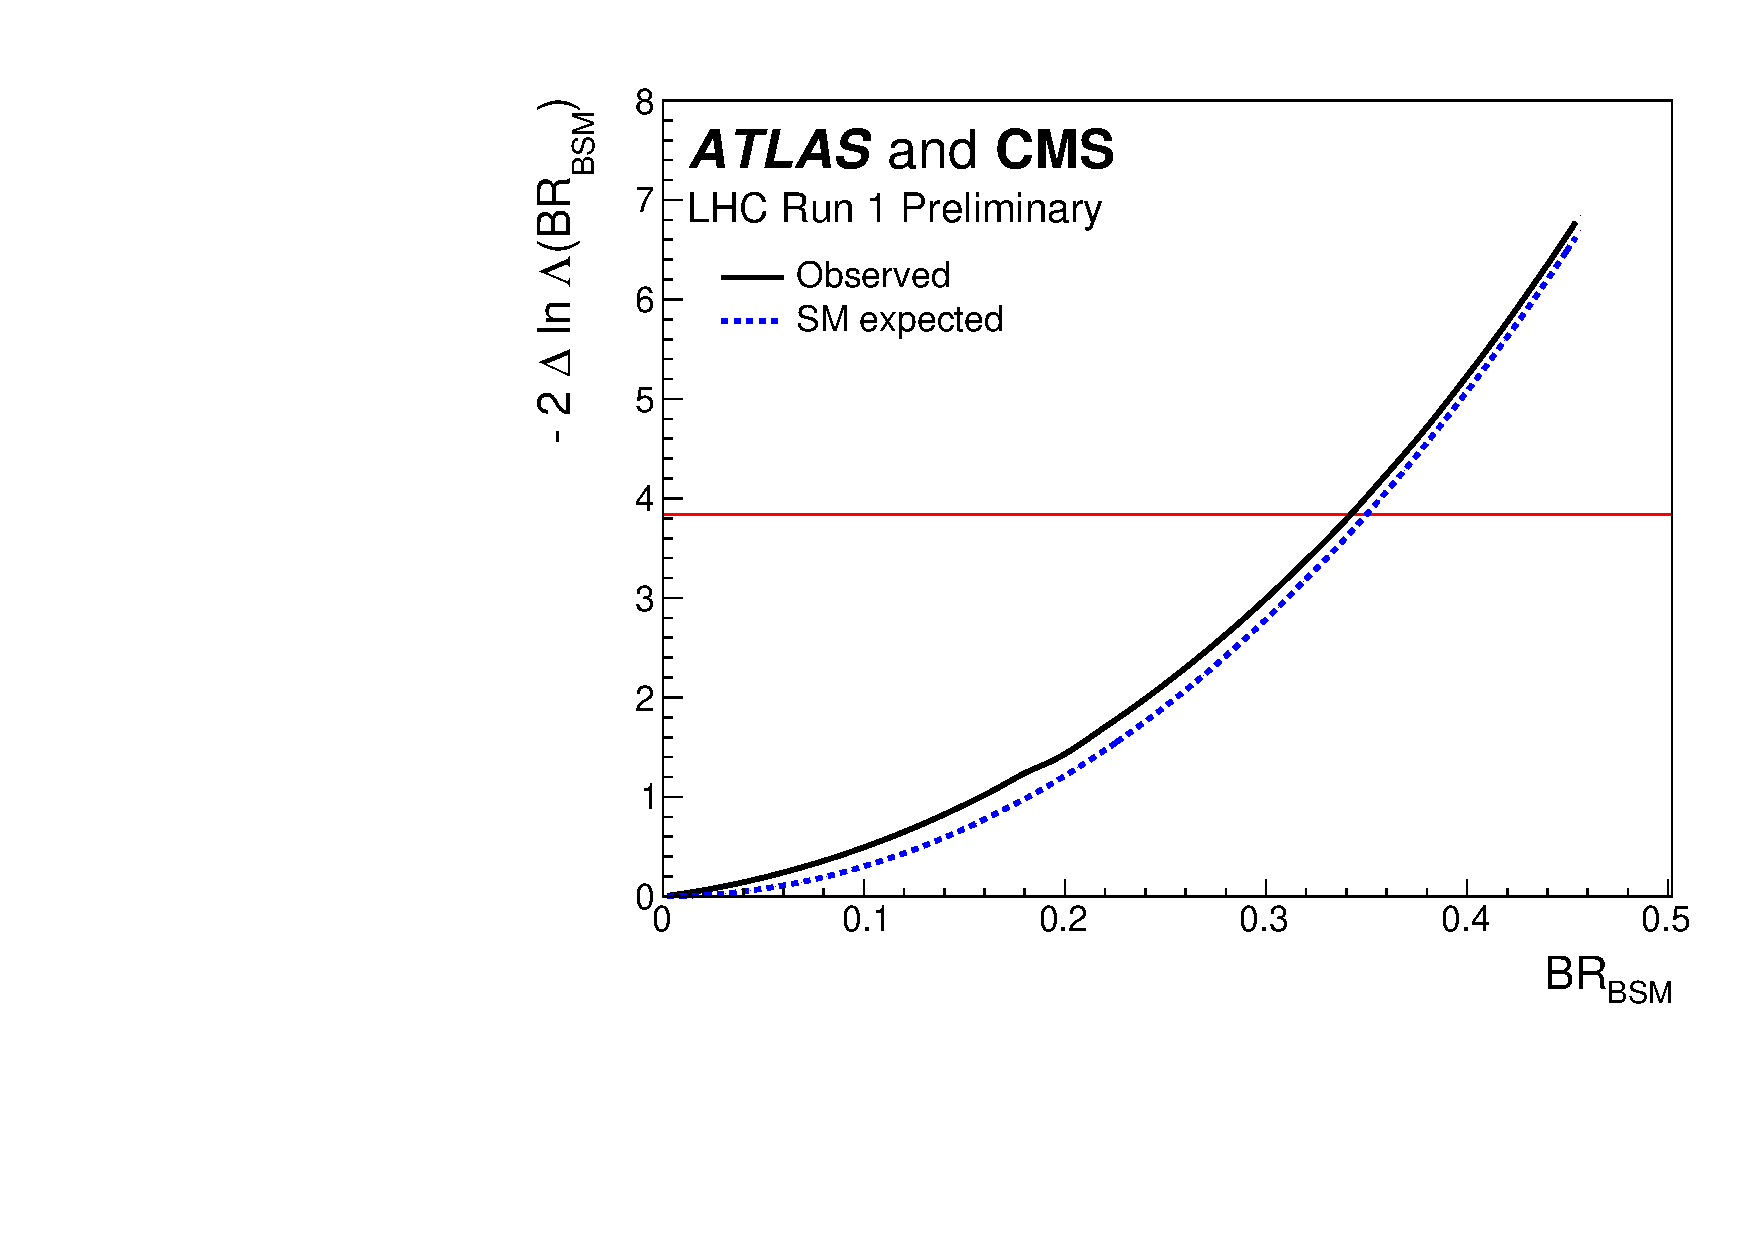
\includegraphics[width=\textwidth]{TalkPics/DM@LHC2016/CMS-PAS-HIG-15-002_Figure_015.pdf}
      \centering
      \scriptsize

      CMS-PAS-HIG-15-002
      
      ATLAS-CONF-2015-044
       \end{columns}
       %??ATLAS or CMS rates of each channel plot
  \end{frame}

  \begin{frame}
    \frametitle{How to search for invisibly decaying Higgs bosons}
    \begin{columns}
      \column{1.06\textwidth}
    \begin{block}{}
      \small
      \begin{itemize}
      \item Look for associated Higgs boson products plus $E_{T}^{miss}$
      \end{itemize}
    \end{block}
    \end{columns}
    \begin{columns}
      \column{.5\textwidth}
      \begin{block}{Production channels}
          \small
          %??ggH, VBF, VH tikz lines to plot if time
          \begin{itemize}
          \item Gluon fusion needs ISR
          \item[-] High rate but difficult final state
          \item VBF %??
          \item[-]
          \item VH %??
          \item[-]
          \end{itemize}
      \end{block}
      \column{.5\textwidth}
      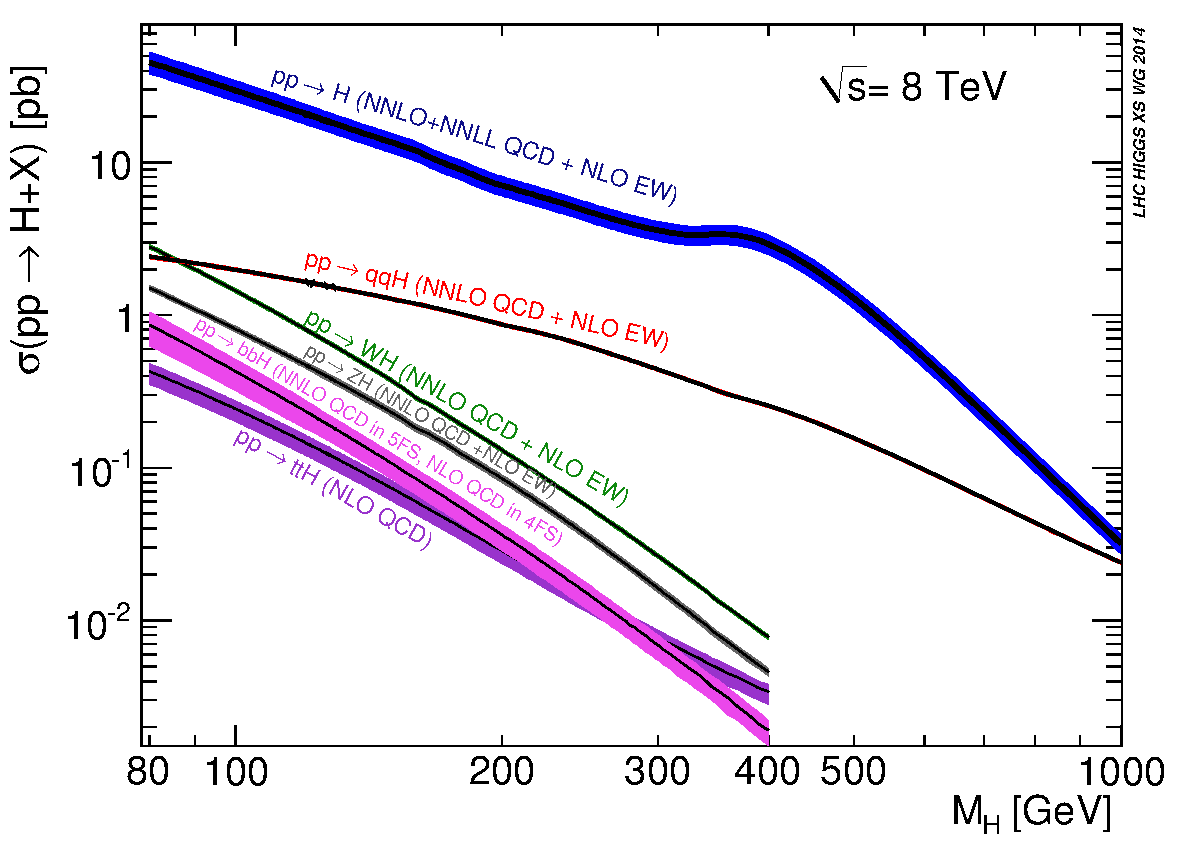
\includegraphics[width=\textwidth]{TalkPics/DM@LHC2016/XS_8TeV-eps-converted-to.pdf}
      \end{columns}
    \end{frame}

  %??ATLAS RUN 1 
  \begin{frame}
    %??V(had)H: http://arxiv.org/abs/1504.04324
    \frametitle{Run 1 ATLAS direct searches - ZH}
    %??search description and limit
  \end{frame}

  \begin{frame}
    %??V(had)H: http://arxiv.org/abs/1504.04324
    \frametitle{Run 1 ATLAS direct searches - V(had)H}
    %??search description and limit
  \end{frame}

  \begin{frame}
    %??http://arxiv.org/pdf/1508.07869v2.pdf
    \frametitle{Run 1 ATLAS direct searches - VBF}
    %??search description and limit mention tying W and Z together
  \end{frame}

  \begin{frame}
    %??http://arxiv.org/pdf/1509.00672v2.pdf (fig 8)
    %??comb with vis
    \frametitle{Run 1 ATLAS direct searches - Combination}
  \end{frame}



  %??CMS Run 1
  \begin{frame}
    %??HIG-13-030
    \frametitle{Run 1 CMS direct searches - ZH}
    \begin{columns}
      %??quick description comb from hig-13-030
    \end{columns}
  \end{frame}

  \begin{frame}
    %??EXO-12-055
    \frametitle{Run 1 CMS direct searches - Monojet}
    \begin{columns}
      %??quick description
      %??fig 8b from pas
    \end{columns}
  \end{frame}

  \begin{frame}
    %??HIG-14-038
    \frametitle{Run 1 CMS direct searches - VBF}
    \begin{columns}
      %??quick description of parked data  
      %??limit plot from hig-14-038
    \end{columns}
  \end{frame}

  \begin{frame}
    %??HIG-15-012
    \frametitle{Run 1 CMS direct searches - Combination}
    \begin{columns}
      %??by category plot
    \end{columns}
  \end{frame}

  %??CMS Run 2
  \begin{frame}
    %??HIG-16-008
    \frametitle{Run 2 CMS direct searches - ZH}
    %??fig 3c, mention move away from mass scans in BR
  \end{frame}

  \begin{frame}
    %??HIG-16-009
    \frametitle{Run 2 CMS direct searches - VBF}
    %??mass scan plot
  \end{frame}
  
  %??HIG-16-009 Combination CMS Run 1 + Run 2
  \begin{frame}
    \frametitle{Run 2 CMS direct searches - Combination}
    %??explain contributing analyses
    %??13 TeV only and 8 TeV+13 TeV category plot
  \end{frame}

  

  %??DM pheno paper
  \begin{frame}
    \frametitle{CMS projections and interpretations}
  \end{frame}

  \begin{frame}
    \frametitle{Summary}
    \label{lastframe}
    \begin{itemize}
    \item 
    \end{itemize}
  \end{frame}
  
\end{fmffile}
\end{document}

